\documentclass[1p]{elsarticle_modified}
%\bibliographystyle{elsarticle-num}

%\usepackage[colorlinks]{hyperref}
%\usepackage{abbrmath_seonhwa} %\Abb, \Ascr, \Acal ,\Abf, \Afrak
\usepackage{amsfonts}
\usepackage{amssymb}
\usepackage{amsmath}
\usepackage{amsthm}
\usepackage{scalefnt}
\usepackage{amsbsy}
\usepackage{kotex}
\usepackage{caption}
\usepackage{subfig}
\usepackage{color}
\usepackage{graphicx}
\usepackage{xcolor} %% white, black, red, green, blue, cyan, magenta, yellow
\usepackage{float}
\usepackage{setspace}
\usepackage{hyperref}

\usepackage{tikz}
\usetikzlibrary{arrows}

\usepackage{multirow}
\usepackage{array} % fixed length table
\usepackage{hhline}

%%%%%%%%%%%%%%%%%%%%%
\makeatletter
\renewcommand*\env@matrix[1][\arraystretch]{%
	\edef\arraystretch{#1}%
	\hskip -\arraycolsep
	\let\@ifnextchar\new@ifnextchar
	\array{*\c@MaxMatrixCols c}}
\makeatother %https://tex.stackexchange.com/questions/14071/how-can-i-increase-the-line-spacing-in-a-matrix
%%%%%%%%%%%%%%%

\usepackage[normalem]{ulem}

\newcommand{\msout}[1]{\ifmmode\text{\sout{\ensuremath{#1}}}\else\sout{#1}\fi}
%SOURCE: \msout is \stkout macro in https://tex.stackexchange.com/questions/20609/strikeout-in-math-mode

\newcommand{\cancel}[1]{
	\ifmmode
	{\color{red}\msout{#1}}
	\else
	{\color{red}\sout{#1}}
	\fi
}

\newcommand{\add}[1]{
	{\color{blue}\uwave{#1}}
}

\newcommand{\replace}[2]{
	\ifmmode
	{\color{red}\msout{#1}}{\color{blue}\uwave{#2}}
	\else
	{\color{red}\sout{#1}}{\color{blue}\uwave{#2}}
	\fi
}

\newcommand{\Sol}{\mathcal{S}} %segment
\newcommand{\D}{D} %diagram
\newcommand{\A}{\mathcal{A}} %arc


%%%%%%%%%%%%%%%%%%%%%%%%%%%%%5 test

\def\sl{\operatorname{\textup{SL}}(2,\Cbb)}
\def\psl{\operatorname{\textup{PSL}}(2,\Cbb)}
\def\quan{\mkern 1mu \triangleright \mkern 1mu}

\theoremstyle{definition}
\newtheorem{thm}{Theorem}[section]
\newtheorem{prop}[thm]{Proposition}
\newtheorem{lem}[thm]{Lemma}
\newtheorem{ques}[thm]{Question}
\newtheorem{cor}[thm]{Corollary}
\newtheorem{defn}[thm]{Definition}
\newtheorem{exam}[thm]{Example}
\newtheorem{rmk}[thm]{Remark}
\newtheorem{alg}[thm]{Algorithm}

\newcommand{\I}{\sqrt{-1}}
\begin{document}

%\begin{frontmatter}
%
%\title{Boundary parabolic representations of knots up to 8 crossings}
%
%%% Group authors per affiliation:
%\author{Yunhi Cho} 
%\address{Department of Mathematics, University of Seoul, Seoul, Korea}
%\ead{yhcho@uos.ac.kr}
%
%
%\author{Seonhwa Kim} %\fnref{s_kim}}
%\address{Center for Geometry and Physics, Institute for Basic Science, Pohang, 37673, Korea}
%\ead{ryeona17@ibs.re.kr}
%
%\author{Hyuk Kim}
%\address{Department of Mathematical Sciences, Seoul National University, Seoul 08826, Korea}
%\ead{hyukkim@snu.ac.kr}
%
%\author{Seokbeom Yoon}
%\address{Department of Mathematical Sciences, Seoul National University, Seoul, 08826,  Korea}
%\ead{sbyoon15@snu.ac.kr}
%
%\begin{abstract}
%We find all boundary parabolic representation of knots up to 8 crossings.
%
%\end{abstract}
%\begin{keyword}
%    \MSC[2010] 57M25 
%\end{keyword}
%
%\end{frontmatter}

%\linenumbers
%\tableofcontents
%
\newcommand\colored[1]{\textcolor{white}{\rule[-0.35ex]{0.8em}{1.4ex}}\kern-0.8em\color{red} #1}%
%\newcommand\colored[1]{\textcolor{white}{ #1}\kern-2.17ex	\textcolor{white}{ #1}\kern-1.81ex	\textcolor{white}{ #1}\kern-2.15ex\color{red}#1	}

{\Large $\underline{12a_{0968}~(K12a_{0968})}$}

\setlength{\tabcolsep}{10pt}
\renewcommand{\arraystretch}{1.6}
\vspace{1cm}\begin{tabular}{m{100pt}>{\centering\arraybackslash}m{274pt}}
\multirow{5}{120pt}{
	\centering
	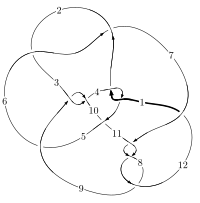
\includegraphics[width=112pt]{../../../GIT/diagram.site/Diagrams/png/1769_12a_0968.png}\\
\ \ \ A knot diagram\footnotemark}&
\allowdisplaybreaks
\textbf{Linearized knot diagam} \\
\cline{2-2}
 &
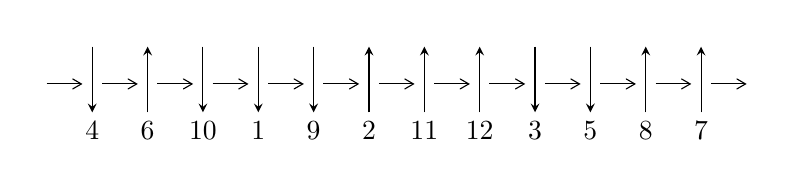
\begin{tikzpicture}[x=20pt, y=17pt]
	% nodes
	\node (C0) at (0, 0) {};
	\node (C1) at (1, 0) {};
	\node (C1U) at (1, +1) {};
	\node (C1D) at (1, -1) {4};

	\node (C2) at (2, 0) {};
	\node (C2U) at (2, +1) {};
	\node (C2D) at (2, -1) {6};

	\node (C3) at (3, 0) {};
	\node (C3U) at (3, +1) {};
	\node (C3D) at (3, -1) {10};

	\node (C4) at (4, 0) {};
	\node (C4U) at (4, +1) {};
	\node (C4D) at (4, -1) {1};

	\node (C5) at (5, 0) {};
	\node (C5U) at (5, +1) {};
	\node (C5D) at (5, -1) {9};

	\node (C6) at (6, 0) {};
	\node (C6U) at (6, +1) {};
	\node (C6D) at (6, -1) {2};

	\node (C7) at (7, 0) {};
	\node (C7U) at (7, +1) {};
	\node (C7D) at (7, -1) {11};

	\node (C8) at (8, 0) {};
	\node (C8U) at (8, +1) {};
	\node (C8D) at (8, -1) {12};

	\node (C9) at (9, 0) {};
	\node (C9U) at (9, +1) {};
	\node (C9D) at (9, -1) {3};

	\node (C10) at (10, 0) {};
	\node (C10U) at (10, +1) {};
	\node (C10D) at (10, -1) {5};

	\node (C11) at (11, 0) {};
	\node (C11U) at (11, +1) {};
	\node (C11D) at (11, -1) {8};

	\node (C12) at (12, 0) {};
	\node (C12U) at (12, +1) {};
	\node (C12D) at (12, -1) {7};
	\node (C13) at (13, 0) {};

	% arrows
	\draw[->,>={angle 60}]
	(C0) edge (C1) (C1) edge (C2) (C2) edge (C3) (C3) edge (C4) (C4) edge (C5) (C5) edge (C6) (C6) edge (C7) (C7) edge (C8) (C8) edge (C9) (C9) edge (C10) (C10) edge (C11) (C11) edge (C12) (C12) edge (C13) ;	\draw[->,>=stealth]
	(C1U) edge (C1D) (C2D) edge (C2U) (C3U) edge (C3D) (C4U) edge (C4D) (C5U) edge (C5D) (C6D) edge (C6U) (C7D) edge (C7U) (C8D) edge (C8U) (C9U) edge (C9D) (C10U) edge (C10D) (C11D) edge (C11U) (C12D) edge (C12U) ;
	\end{tikzpicture} \\
\hhline{~~} \\& 
\textbf{Solving Sequence} \\ \cline{2-2} 
 &
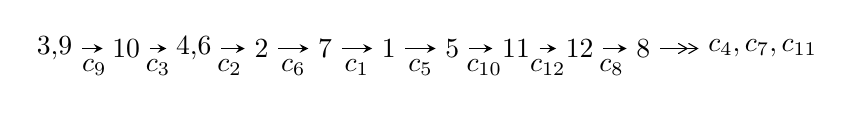
\begin{tikzpicture}[x=23pt, y=7pt]
	% node
	\node (A0) at (-1/8, 0) {3,9};
	\node (A1) at (1, 0) {10};
	\node (A2) at (33/16, 0) {4,6};
	\node (A3) at (25/8, 0) {2};
	\node (A4) at (33/8, 0) {7};
	\node (A5) at (41/8, 0) {1};
	\node (A6) at (49/8, 0) {5};
	\node (A7) at (57/8, 0) {11};
	\node (A8) at (65/8, 0) {12};
	\node (A9) at (73/8, 0) {8};
	\node (C1) at (1/2, -1) {$c_{9}$};
	\node (C2) at (3/2, -1) {$c_{3}$};
	\node (C3) at (21/8, -1) {$c_{2}$};
	\node (C4) at (29/8, -1) {$c_{6}$};
	\node (C5) at (37/8, -1) {$c_{1}$};
	\node (C6) at (45/8, -1) {$c_{5}$};
	\node (C7) at (53/8, -1) {$c_{10}$};
	\node (C8) at (61/8, -1) {$c_{12}$};
	\node (C9) at (69/8, -1) {$c_{8}$};
	\node (A10) at (11, 0) {$c_{4},c_{7},c_{11}$};

	% edge
	\draw[->,>=stealth]	
	(A0) edge (A1) (A1) edge (A2) (A2) edge (A3) (A3) edge (A4) (A4) edge (A5) (A5) edge (A6) (A6) edge (A7) (A7) edge (A8) (A8) edge (A9) ;
	\draw[->>,>={angle 60}]	
	(A9) edge (A10);
\end{tikzpicture} \\ 

\end{tabular} \\

\footnotetext{
The image of knot diagram is generated by the software ``\textbf{Draw programme}" developed by Andrew Bartholomew(\url{http://www.layer8.co.uk/maths/draw/index.htm\#Running-draw}), where we modified some parts for our purpose(\url{https://github.com/CATsTAILs/LinksPainter}).
}\phantom \\ \newline 
\centering \textbf{Ideals for irreducible components\footnotemark of $X_{\text{par}}$} 
 
\begin{align*}
I^u_{1}&=\langle 
1.66735\times10^{500} u^{123}-2.11747\times10^{498} u^{122}+\cdots+1.13618\times10^{500} b+5.33111\times10^{503},\\
\phantom{I^u_{1}}&\phantom{= \langle  }-7.52490\times10^{503} u^{123}-1.24524\times10^{502} u^{122}+\cdots+3.79142\times10^{503} a-2.44838\times10^{507},\\
\phantom{I^u_{1}}&\phantom{= \langle  }u^{124}+u^{123}+\cdots+6267 u+3337\rangle \\
I^u_{2}&=\langle 
146398895 u^{27}-49300484 u^{26}+\cdots+30684719 b+180392163,\\
\phantom{I^u_{2}}&\phantom{= \langle  }345321576 u^{27}-131091679 u^{26}+\cdots+30684719 a+749968064,\;u^{28}-9 u^{26}+\cdots+3 u+1\rangle \\
\\
\end{align*}
\raggedright * 2 irreducible components of $\dim_{\mathbb{C}}=0$, with total 152 representations.\\
\footnotetext{All coefficients of polynomials are rational numbers. But the coefficients are sometimes approximated in decimal forms when there is not enough margin.}
\newpage
\renewcommand{\arraystretch}{1}
\centering \section*{I. $I^u_{1}= \langle 1.67\times10^{500} u^{123}-2.12\times10^{498} u^{122}+\cdots+1.14\times10^{500} b+5.33\times10^{503},\;-7.52\times10^{503} u^{123}-1.25\times10^{502} u^{122}+\cdots+3.79\times10^{503} a-2.45\times10^{507},\;u^{124}+u^{123}+\cdots+6267 u+3337 \rangle$}
\flushleft \textbf{(i) Arc colorings}\\
\begin{tabular}{m{7pt} m{180pt} m{7pt} m{180pt} }
\flushright $a_{3}=$&$\begin{pmatrix}0\\u\end{pmatrix}$ \\
\flushright $a_{9}=$&$\begin{pmatrix}1\\0\end{pmatrix}$ \\
\flushright $a_{10}=$&$\begin{pmatrix}1\\u^2\end{pmatrix}$ \\
\flushright $a_{4}=$&$\begin{pmatrix}- u\\- u^3+u\end{pmatrix}$ \\
\flushright $a_{6}=$&$\begin{pmatrix}1.98472 u^{123}+0.0328437 u^{122}+\cdots+5699.24 u+6457.70\\-1.46751 u^{123}+0.0186369 u^{122}+\cdots-4276.35 u-4692.15\end{pmatrix}$ \\
\flushright $a_{2}=$&$\begin{pmatrix}-1.69518 u^{123}+0.130301 u^{122}+\cdots-4860.86 u-5060.88\\-1.93539 u^{123}+0.0534685 u^{122}+\cdots-5542.57 u-6049.77\end{pmatrix}$ \\
\flushright $a_{7}=$&$\begin{pmatrix}-0.0614829 u^{123}-0.418132 u^{122}+\cdots-260.898 u-1428.36\\0.509867 u^{123}-0.144487 u^{122}+\cdots+1458.46 u+1233.81\end{pmatrix}$ \\
\flushright $a_{1}=$&$\begin{pmatrix}-3.50486 u^{123}+0.178179 u^{122}+\cdots-10051.2 u-10731.9\\-2.06520 u^{123}+0.0248781 u^{122}+\cdots-5954.65 u-6577.43\end{pmatrix}$ \\
\flushright $a_{5}=$&$\begin{pmatrix}0.517208 u^{123}+0.0514805 u^{122}+\cdots+1422.89 u+1765.54\\-1.46751 u^{123}+0.0186369 u^{122}+\cdots-4276.35 u-4692.15\end{pmatrix}$ \\
\flushright $a_{11}=$&$\begin{pmatrix}3.37498 u^{123}-0.224652 u^{122}+\cdots+10242.0 u+10695.4\\1.37358 u^{123}-0.0868308 u^{122}+\cdots+4199.78 u+4397.25\end{pmatrix}$ \\
\flushright $a_{12}=$&$\begin{pmatrix}1.98546 u^{123}-0.0457094 u^{122}+\cdots+5925.96 u+6443.94\\-0.589160 u^{123}+0.142648 u^{122}+\cdots-1756.81 u-1539.59\end{pmatrix}$ \\
\flushright $a_{8}=$&$\begin{pmatrix}-2.96853 u^{123}-0.0341607 u^{122}+\cdots-8928.85 u-9979.19\\-0.253373 u^{123}-0.109983 u^{122}+\cdots-787.410 u-1204.28\end{pmatrix}$\\&\end{tabular}
\flushleft \textbf{(ii) Obstruction class $= -1$}\\~\\
\flushleft \textbf{(iii) Cusp Shapes $= 0.783501 u^{123}-0.0743194 u^{122}+\cdots+2037.91 u+2088.12$}\\~\\
\newpage\renewcommand{\arraystretch}{1}
\flushleft \textbf{(iv) u-Polynomials at the component}\newline \\
\begin{tabular}{m{50pt}|m{274pt}}
Crossings & \hspace{64pt}u-Polynomials at each crossing \\
\hline $$\begin{aligned}c_{1},c_{4}\end{aligned}$$&$\begin{aligned}
&u^{124}-6 u^{123}+\cdots-1685 u+409
\end{aligned}$\\
\hline $$\begin{aligned}c_{2},c_{6}\end{aligned}$$&$\begin{aligned}
&u^{124}-2 u^{123}+\cdots+4203615 u+452717
\end{aligned}$\\
\hline $$\begin{aligned}c_{3},c_{9}\end{aligned}$$&$\begin{aligned}
&u^{124}+u^{123}+\cdots+6267 u+3337
\end{aligned}$\\
\hline $$\begin{aligned}c_{5}\end{aligned}$$&$\begin{aligned}
&u^{124}+3 u^{123}+\cdots+57474466 u+17460809
\end{aligned}$\\
\hline $$\begin{aligned}c_{7},c_{8},c_{11}\end{aligned}$$&$\begin{aligned}
&u^{124}-3 u^{123}+\cdots+78 u+17
\end{aligned}$\\
\hline $$\begin{aligned}c_{10}\end{aligned}$$&$\begin{aligned}
&u^{124}- u^{123}+\cdots-4921 u+587
\end{aligned}$\\
\hline $$\begin{aligned}c_{12}\end{aligned}$$&$\begin{aligned}
&u^{124}+9 u^{123}+\cdots-252952 u-25823
\end{aligned}$\\
\hline
\end{tabular}\\~\\
\newpage\renewcommand{\arraystretch}{1}
\flushleft \textbf{(v) Riley Polynomials at the component}\newline \\
\begin{tabular}{m{50pt}|m{274pt}}
Crossings & \hspace{64pt}Riley Polynomials at each crossing \\
\hline $$\begin{aligned}c_{1},c_{4}\end{aligned}$$&$\begin{aligned}
&y^{124}+72 y^{123}+\cdots+9830777 y+167281
\end{aligned}$\\
\hline $$\begin{aligned}c_{2},c_{6}\end{aligned}$$&$\begin{aligned}
&y^{124}+94 y^{123}+\cdots+2080269273415 y+204952682089
\end{aligned}$\\
\hline $$\begin{aligned}c_{3},c_{9}\end{aligned}$$&$\begin{aligned}
&y^{124}-85 y^{123}+\cdots-217417697 y+11135569
\end{aligned}$\\
\hline $$\begin{aligned}c_{5}\end{aligned}$$&$\begin{aligned}
&y^{124}-49 y^{123}+\cdots-10380445673668428 y+304879850934481
\end{aligned}$\\
\hline $$\begin{aligned}c_{7},c_{8},c_{11}\end{aligned}$$&$\begin{aligned}
&y^{124}-113 y^{123}+\cdots+8842 y+289
\end{aligned}$\\
\hline $$\begin{aligned}c_{10}\end{aligned}$$&$\begin{aligned}
&y^{124}-11 y^{123}+\cdots-15729395 y+344569
\end{aligned}$\\
\hline $$\begin{aligned}c_{12}\end{aligned}$$&$\begin{aligned}
&y^{124}+19 y^{123}+\cdots-40988713052 y+666827329
\end{aligned}$\\
\hline
\end{tabular}\\~\\
\newpage\flushleft \textbf{(vi) Complex Volumes and Cusp Shapes}
$$\begin{array}{c|c|c}  
\text{Solutions to }I^u_{1}& \I (\text{vol} + \sqrt{-1}CS) & \text{Cusp shape}\\
 \hline 
\begin{aligned}
u &= \phantom{-}0.751395 + 0.647947 I \\
a &= -0.444423 - 0.851288 I \\
b &= \phantom{-}1.43800 - 0.30287 I\end{aligned}
 & \phantom{-}0.35757 - 2.52458 I & \phantom{-0.000000 } 0 \\ \hline\begin{aligned}
u &= \phantom{-}0.751395 - 0.647947 I \\
a &= -0.444423 + 0.851288 I \\
b &= \phantom{-}1.43800 + 0.30287 I\end{aligned}
 & \phantom{-}0.35757 + 2.52458 I & \phantom{-0.000000 } 0 \\ \hline\begin{aligned}
u &= \phantom{-}1.017530 + 0.090414 I \\
a &= \phantom{-}0.138485 + 0.982190 I \\
b &= \phantom{-}1.20561 - 1.66871 I\end{aligned}
 & \phantom{-}4.48519 + 0.42117 I & \phantom{-0.000000 } 0 \\ \hline\begin{aligned}
u &= \phantom{-}1.017530 - 0.090414 I \\
a &= \phantom{-}0.138485 - 0.982190 I \\
b &= \phantom{-}1.20561 + 1.66871 I\end{aligned}
 & \phantom{-}4.48519 - 0.42117 I & \phantom{-0.000000 } 0 \\ \hline\begin{aligned}
u &= -0.856183 + 0.561569 I \\
a &= \phantom{-}0.579030 - 0.243502 I \\
b &= -0.717906 - 0.769695 I\end{aligned}
 & -0.64210 + 2.71262 I & \phantom{-0.000000 } 0 \\ \hline\begin{aligned}
u &= -0.856183 - 0.561569 I \\
a &= \phantom{-}0.579030 + 0.243502 I \\
b &= -0.717906 + 0.769695 I\end{aligned}
 & -0.64210 - 2.71262 I & \phantom{-0.000000 } 0 \\ \hline\begin{aligned}
u &= -0.379617 + 0.961102 I \\
a &= -0.292892 + 0.684607 I \\
b &= -0.072348 - 0.810126 I\end{aligned}
 & \phantom{-}9.86516 + 1.82868 I & \phantom{-0.000000 } 0 \\ \hline\begin{aligned}
u &= -0.379617 - 0.961102 I \\
a &= -0.292892 - 0.684607 I \\
b &= -0.072348 + 0.810126 I\end{aligned}
 & \phantom{-}9.86516 - 1.82868 I & \phantom{-0.000000 } 0 \\ \hline\begin{aligned}
u &= -0.686990 + 0.673145 I \\
a &= \phantom{-}0.450248 - 1.025700 I \\
b &= -1.59802 - 0.06875 I\end{aligned}
 & \phantom{-}4.72490 + 5.19947 I & \phantom{-0.000000 } 0 \\ \hline\begin{aligned}
u &= -0.686990 - 0.673145 I \\
a &= \phantom{-}0.450248 + 1.025700 I \\
b &= -1.59802 + 0.06875 I\end{aligned}
 & \phantom{-}4.72490 - 5.19947 I & \phantom{-0.000000 } 0\\
 \hline 
 \end{array}$$\newpage$$\begin{array}{c|c|c}  
\text{Solutions to }I^u_{1}& \I (\text{vol} + \sqrt{-1}CS) & \text{Cusp shape}\\
 \hline 
\begin{aligned}
u &= -0.801645 + 0.676898 I \\
a &= \phantom{-}0.595452 - 0.760437 I \\
b &= -1.49274 - 0.58807 I\end{aligned}
 & \phantom{-}4.44911 - 0.03429 I & \phantom{-0.000000 } 0 \\ \hline\begin{aligned}
u &= -0.801645 - 0.676898 I \\
a &= \phantom{-}0.595452 + 0.760437 I \\
b &= -1.49274 + 0.58807 I\end{aligned}
 & \phantom{-}4.44911 + 0.03429 I & \phantom{-0.000000 } 0 \\ \hline\begin{aligned}
u &= -0.183995 + 0.923140 I \\
a &= \phantom{-}1.287490 - 0.218341 I \\
b &= -0.996040 + 0.273161 I\end{aligned}
 & -1.74802 - 1.57494 I & \phantom{-0.000000 } 0 \\ \hline\begin{aligned}
u &= -0.183995 - 0.923140 I \\
a &= \phantom{-}1.287490 + 0.218341 I \\
b &= -0.996040 - 0.273161 I\end{aligned}
 & -1.74802 + 1.57494 I & \phantom{-0.000000 } 0 \\ \hline\begin{aligned}
u &= -1.046320 + 0.166367 I \\
a &= \phantom{-}0.060385 + 0.948348 I \\
b &= -0.20035 - 2.35004 I\end{aligned}
 & \phantom{-}3.24681 + 8.29685 I & \phantom{-0.000000 } 0 \\ \hline\begin{aligned}
u &= -1.046320 - 0.166367 I \\
a &= \phantom{-}0.060385 - 0.948348 I \\
b &= -0.20035 + 2.35004 I\end{aligned}
 & \phantom{-}3.24681 - 8.29685 I & \phantom{-0.000000 } 0 \\ \hline\begin{aligned}
u &= -1.063870 + 0.099118 I \\
a &= -0.42909 - 1.69946 I \\
b &= -0.929060 + 0.381333 I\end{aligned}
 & -3.04067 + 4.79725 I & \phantom{-0.000000 } 0 \\ \hline\begin{aligned}
u &= -1.063870 - 0.099118 I \\
a &= -0.42909 + 1.69946 I \\
b &= -0.929060 - 0.381333 I\end{aligned}
 & -3.04067 - 4.79725 I & \phantom{-0.000000 } 0 \\ \hline\begin{aligned}
u &= \phantom{-}0.885111 + 0.605177 I \\
a &= -0.681560 - 0.390823 I \\
b &= \phantom{-}0.940572 - 0.944198 I\end{aligned}
 & \phantom{-}3.78465 - 5.84346 I & \phantom{-0.000000 } 0 \\ \hline\begin{aligned}
u &= \phantom{-}0.885111 - 0.605177 I \\
a &= -0.681560 + 0.390823 I \\
b &= \phantom{-}0.940572 + 0.944198 I\end{aligned}
 & \phantom{-}3.78465 + 5.84346 I & \phantom{-0.000000 } 0\\
 \hline 
 \end{array}$$\newpage$$\begin{array}{c|c|c}  
\text{Solutions to }I^u_{1}& \I (\text{vol} + \sqrt{-1}CS) & \text{Cusp shape}\\
 \hline 
\begin{aligned}
u &= \phantom{-}0.997576 + 0.396495 I \\
a &= \phantom{-}0.662400 - 0.603344 I \\
b &= \phantom{-}0.888350 + 0.250860 I\end{aligned}
 & \phantom{-}1.29894 - 3.71169 I & \phantom{-0.000000 } 0 \\ \hline\begin{aligned}
u &= \phantom{-}0.997576 - 0.396495 I \\
a &= \phantom{-}0.662400 + 0.603344 I \\
b &= \phantom{-}0.888350 - 0.250860 I\end{aligned}
 & \phantom{-}1.29894 + 3.71169 I & \phantom{-0.000000 } 0 \\ \hline\begin{aligned}
u &= -1.073680 + 0.087462 I \\
a &= -0.037092 + 1.086680 I \\
b &= -0.60112 - 1.44378 I\end{aligned}
 & -1.49679 + 1.67439 I & \phantom{-0.000000 } 0 \\ \hline\begin{aligned}
u &= -1.073680 - 0.087462 I \\
a &= -0.037092 - 1.086680 I \\
b &= -0.60112 + 1.44378 I\end{aligned}
 & -1.49679 - 1.67439 I & \phantom{-0.000000 } 0 \\ \hline\begin{aligned}
u &= \phantom{-}1.085070 + 0.087802 I \\
a &= \phantom{-}0.22542 - 1.66536 I \\
b &= \phantom{-}0.833203 + 0.405992 I\end{aligned}
 & -7.03932 - 0.59794 I & \phantom{-0.000000 } 0 \\ \hline\begin{aligned}
u &= \phantom{-}1.085070 - 0.087802 I \\
a &= \phantom{-}0.22542 + 1.66536 I \\
b &= \phantom{-}0.833203 - 0.405992 I\end{aligned}
 & -7.03932 + 0.59794 I & \phantom{-0.000000 } 0 \\ \hline\begin{aligned}
u &= \phantom{-}1.078720 + 0.151683 I \\
a &= -0.059149 + 1.008330 I \\
b &= \phantom{-}0.13577 - 1.91283 I\end{aligned}
 & -2.21566 - 5.13599 I & \phantom{-0.000000 } 0 \\ \hline\begin{aligned}
u &= \phantom{-}1.078720 - 0.151683 I \\
a &= -0.059149 - 1.008330 I \\
b &= \phantom{-}0.13577 + 1.91283 I\end{aligned}
 & -2.21566 + 5.13599 I & \phantom{-0.000000 } 0 \\ \hline\begin{aligned}
u &= \phantom{-}0.816050 + 0.330070 I \\
a &= -0.731451 + 0.044798 I \\
b &= \phantom{-}0.183690 - 0.541400 I\end{aligned}
 & \phantom{-}2.65243 + 0.13673 I & \phantom{-0.000000 } 0 \\ \hline\begin{aligned}
u &= \phantom{-}0.816050 - 0.330070 I \\
a &= -0.731451 - 0.044798 I \\
b &= \phantom{-}0.183690 + 0.541400 I\end{aligned}
 & \phantom{-}2.65243 - 0.13673 I & \phantom{-0.000000 } 0\\
 \hline 
 \end{array}$$\newpage$$\begin{array}{c|c|c}  
\text{Solutions to }I^u_{1}& \I (\text{vol} + \sqrt{-1}CS) & \text{Cusp shape}\\
 \hline 
\begin{aligned}
u &= -1.121600 + 0.075195 I \\
a &= -0.03111 - 1.58714 I \\
b &= -0.679209 + 0.413456 I\end{aligned}
 & -3.25272 - 3.53201 I & \phantom{-0.000000 } 0 \\ \hline\begin{aligned}
u &= -1.121600 - 0.075195 I \\
a &= -0.03111 + 1.58714 I \\
b &= -0.679209 - 0.413456 I\end{aligned}
 & -3.25272 + 3.53201 I & \phantom{-0.000000 } 0 \\ \hline\begin{aligned}
u &= \phantom{-}1.078790 + 0.328127 I \\
a &= \phantom{-}0.959816 - 0.631273 I \\
b &= \phantom{-}0.963005 + 0.378001 I\end{aligned}
 & \phantom{-}1.16463 - 3.54205 I & \phantom{-0.000000 } 0 \\ \hline\begin{aligned}
u &= \phantom{-}1.078790 - 0.328127 I \\
a &= \phantom{-}0.959816 + 0.631273 I \\
b &= \phantom{-}0.963005 - 0.378001 I\end{aligned}
 & \phantom{-}1.16463 + 3.54205 I & \phantom{-0.000000 } 0 \\ \hline\begin{aligned}
u &= -1.13389\phantom{ +0.000000I} \\
a &= \phantom{-}0.573544\phantom{ +0.000000I} \\
b &= \phantom{-}0.904582\phantom{ +0.000000I}\end{aligned}
 & -2.33630\phantom{ +0.000000I} & \phantom{-0.000000 } 0 \\ \hline\begin{aligned}
u &= \phantom{-}0.456626 + 0.702250 I \\
a &= -0.149831 + 0.709393 I \\
b &= \phantom{-}0.430576 - 0.684536 I\end{aligned}
 & \phantom{-}3.00312 - 0.38713 I & \phantom{-0.000000 } 0 \\ \hline\begin{aligned}
u &= \phantom{-}0.456626 - 0.702250 I \\
a &= -0.149831 - 0.709393 I \\
b &= \phantom{-}0.430576 + 0.684536 I\end{aligned}
 & \phantom{-}3.00312 + 0.38713 I & \phantom{-0.000000 } 0 \\ \hline\begin{aligned}
u &= \phantom{-}0.060198 + 0.827365 I \\
a &= -1.49574 - 0.23920 I \\
b &= \phantom{-}1.015420 + 0.502709 I\end{aligned}
 & -4.81453 - 2.53246 I & \phantom{-0.000000 } 0 \\ \hline\begin{aligned}
u &= \phantom{-}0.060198 - 0.827365 I \\
a &= -1.49574 + 0.23920 I \\
b &= \phantom{-}1.015420 - 0.502709 I\end{aligned}
 & -4.81453 + 2.53246 I & \phantom{-0.000000 } 0 \\ \hline\begin{aligned}
u &= -1.20811\phantom{ +0.000000I} \\
a &= \phantom{-}0.450878\phantom{ +0.000000I} \\
b &= \phantom{-}1.26931\phantom{ +0.000000I}\end{aligned}
 & -2.16439\phantom{ +0.000000I} & \phantom{-0.000000 } 0\\
 \hline 
 \end{array}$$\newpage$$\begin{array}{c|c|c}  
\text{Solutions to }I^u_{1}& \I (\text{vol} + \sqrt{-1}CS) & \text{Cusp shape}\\
 \hline 
\begin{aligned}
u &= -1.155800 + 0.352764 I \\
a &= -1.087770 - 0.415277 I \\
b &= -0.936075 + 0.510536 I\end{aligned}
 & -1.26636 + 7.34053 I & \phantom{-0.000000 } 0 \\ \hline\begin{aligned}
u &= -1.155800 - 0.352764 I \\
a &= -1.087770 + 0.415277 I \\
b &= -0.936075 - 0.510536 I\end{aligned}
 & -1.26636 - 7.34053 I & \phantom{-0.000000 } 0 \\ \hline\begin{aligned}
u &= \phantom{-}0.024937 + 0.790745 I \\
a &= \phantom{-}1.62489 - 0.21735 I \\
b &= -1.012460 + 0.682595 I\end{aligned}
 & -0.24714 + 6.43951 I & \phantom{-0.000000 } 0 \\ \hline\begin{aligned}
u &= \phantom{-}0.024937 - 0.790745 I \\
a &= \phantom{-}1.62489 + 0.21735 I \\
b &= -1.012460 - 0.682595 I\end{aligned}
 & -0.24714 - 6.43951 I & \phantom{-0.000000 } 0 \\ \hline\begin{aligned}
u &= \phantom{-}1.215660 + 0.123822 I \\
a &= -0.551505 + 0.226101 I \\
b &= -1.069120 - 0.575509 I\end{aligned}
 & -4.29478 - 2.92680 I & \phantom{-0.000000 } 0 \\ \hline\begin{aligned}
u &= \phantom{-}1.215660 - 0.123822 I \\
a &= -0.551505 - 0.226101 I \\
b &= -1.069120 + 0.575509 I\end{aligned}
 & -4.29478 + 2.92680 I & \phantom{-0.000000 } 0 \\ \hline\begin{aligned}
u &= -0.757982 + 0.159362 I \\
a &= -0.588970 - 1.182140 I \\
b &= -1.167610 + 0.052228 I\end{aligned}
 & -0.023464 + 1.133320 I & \phantom{-0.000000 } 0 \\ \hline\begin{aligned}
u &= -0.757982 - 0.159362 I \\
a &= -0.588970 + 1.182140 I \\
b &= -1.167610 - 0.052228 I\end{aligned}
 & -0.023464 - 1.133320 I & \phantom{-0.000000 } 0 \\ \hline\begin{aligned}
u &= \phantom{-}0.033712 + 1.231080 I \\
a &= \phantom{-}0.975403 + 0.396561 I \\
b &= -1.014710 - 0.615162 I\end{aligned}
 & \phantom{-}3.73079 - 12.02730 I & \phantom{-0.000000 } 0 \\ \hline\begin{aligned}
u &= \phantom{-}0.033712 - 1.231080 I \\
a &= \phantom{-}0.975403 - 0.396561 I \\
b &= -1.014710 + 0.615162 I\end{aligned}
 & \phantom{-}3.73079 + 12.02730 I & \phantom{-0.000000 } 0\\
 \hline 
 \end{array}$$\newpage$$\begin{array}{c|c|c}  
\text{Solutions to }I^u_{1}& \I (\text{vol} + \sqrt{-1}CS) & \text{Cusp shape}\\
 \hline 
\begin{aligned}
u &= \phantom{-}0.766142 + 0.044296 I \\
a &= \phantom{-}0.787040 + 1.002180 I \\
b &= \phantom{-}1.56690 + 0.24167 I\end{aligned}
 & \phantom{-}5.29105 - 1.35557 I & \phantom{-0.000000 } 0 \\ \hline\begin{aligned}
u &= \phantom{-}0.766142 - 0.044296 I \\
a &= \phantom{-}0.787040 - 1.002180 I \\
b &= \phantom{-}1.56690 - 0.24167 I\end{aligned}
 & \phantom{-}5.29105 + 1.35557 I & \phantom{-0.000000 } 0 \\ \hline\begin{aligned}
u &= -1.218500 + 0.200633 I \\
a &= \phantom{-}0.677065 + 0.296816 I \\
b &= \phantom{-}0.967920 - 0.786297 I\end{aligned}
 & \phantom{-}0.59788 + 6.18648 I & \phantom{-0.000000 } 0 \\ \hline\begin{aligned}
u &= -1.218500 - 0.200633 I \\
a &= \phantom{-}0.677065 - 0.296816 I \\
b &= \phantom{-}0.967920 + 0.786297 I\end{aligned}
 & \phantom{-}0.59788 - 6.18648 I & \phantom{-0.000000 } 0 \\ \hline\begin{aligned}
u &= -1.209420 + 0.291333 I \\
a &= \phantom{-}0.146444 + 1.000370 I \\
b &= \phantom{-}1.12628 - 1.36689 I\end{aligned}
 & -0.25642 + 4.13332 I & \phantom{-0.000000 } 0 \\ \hline\begin{aligned}
u &= -1.209420 - 0.291333 I \\
a &= \phantom{-}0.146444 - 1.000370 I \\
b &= \phantom{-}1.12628 + 1.36689 I\end{aligned}
 & -0.25642 - 4.13332 I & \phantom{-0.000000 } 0 \\ \hline\begin{aligned}
u &= \phantom{-}1.190710 + 0.364499 I \\
a &= \phantom{-}1.130320 - 0.313228 I \\
b &= \phantom{-}0.922403 + 0.588108 I\end{aligned}
 & \phantom{-}3.69884 - 11.19260 I & \phantom{-0.000000 } 0 \\ \hline\begin{aligned}
u &= \phantom{-}1.190710 - 0.364499 I \\
a &= \phantom{-}1.130320 + 0.313228 I \\
b &= \phantom{-}0.922403 - 0.588108 I\end{aligned}
 & \phantom{-}3.69884 + 11.19260 I & \phantom{-0.000000 } 0 \\ \hline\begin{aligned}
u &= -0.002259 + 1.248730 I \\
a &= -0.972254 + 0.309604 I \\
b &= \phantom{-}0.997384 - 0.473808 I\end{aligned}
 & -1.72579 + 7.75822 I & \phantom{-0.000000 } 0 \\ \hline\begin{aligned}
u &= -0.002259 - 1.248730 I \\
a &= -0.972254 - 0.309604 I \\
b &= \phantom{-}0.997384 + 0.473808 I\end{aligned}
 & -1.72579 - 7.75822 I & \phantom{-0.000000 } 0\\
 \hline 
 \end{array}$$\newpage$$\begin{array}{c|c|c}  
\text{Solutions to }I^u_{1}& \I (\text{vol} + \sqrt{-1}CS) & \text{Cusp shape}\\
 \hline 
\begin{aligned}
u &= -1.137090 + 0.526599 I \\
a &= -0.726318 - 0.134812 I \\
b &= -0.575613 + 0.413199 I\end{aligned}
 & \phantom{-}7.42382 + 3.42825 I & \phantom{-0.000000 } 0 \\ \hline\begin{aligned}
u &= -1.137090 - 0.526599 I \\
a &= -0.726318 + 0.134812 I \\
b &= -0.575613 - 0.413199 I\end{aligned}
 & \phantom{-}7.42382 - 3.42825 I & \phantom{-0.000000 } 0 \\ \hline\begin{aligned}
u &= \phantom{-}0.457479 + 0.580364 I \\
a &= -0.285439 - 1.349160 I \\
b &= \phantom{-}1.176500 + 0.506816 I\end{aligned}
 & \phantom{-}4.73492 + 1.24675 I & \phantom{-0.000000 } 0 \\ \hline\begin{aligned}
u &= \phantom{-}0.457479 - 0.580364 I \\
a &= -0.285439 + 1.349160 I \\
b &= \phantom{-}1.176500 - 0.506816 I\end{aligned}
 & \phantom{-}4.73492 - 1.24675 I & \phantom{-0.000000 } 0 \\ \hline\begin{aligned}
u &= \phantom{-}0.636864 + 0.373962 I \\
a &= -0.767069 + 0.192017 I \\
b &= \phantom{-}0.428250 - 0.397915 I\end{aligned}
 & \phantom{-}2.62564 + 0.12831 I & \phantom{-0.000000 } 0 \\ \hline\begin{aligned}
u &= \phantom{-}0.636864 - 0.373962 I \\
a &= -0.767069 - 0.192017 I \\
b &= \phantom{-}0.428250 + 0.397915 I\end{aligned}
 & \phantom{-}2.62564 - 0.12831 I & \phantom{-0.000000 } 0 \\ \hline\begin{aligned}
u &= \phantom{-}0.206329 + 0.680251 I \\
a &= \phantom{-}0.030600 + 1.250090 I \\
b &= \phantom{-}0.625464 - 1.042900 I\end{aligned}
 & \phantom{-}6.75201 + 7.26759 I & \phantom{-}7.05707 - 3.65536 I \\ \hline\begin{aligned}
u &= \phantom{-}0.206329 - 0.680251 I \\
a &= \phantom{-}0.030600 - 1.250090 I \\
b &= \phantom{-}0.625464 + 1.042900 I\end{aligned}
 & \phantom{-}6.75201 - 7.26759 I & \phantom{-}7.05707 + 3.65536 I \\ \hline\begin{aligned}
u &= -0.285517 + 0.647666 I \\
a &= \phantom{-}0.147525 + 1.123350 I \\
b &= -0.608234 - 0.879743 I\end{aligned}
 & \phantom{-}1.43374 - 3.53123 I & \phantom{-}2.85137 + 3.03656 I \\ \hline\begin{aligned}
u &= -0.285517 - 0.647666 I \\
a &= \phantom{-}0.147525 - 1.123350 I \\
b &= -0.608234 + 0.879743 I\end{aligned}
 & \phantom{-}1.43374 + 3.53123 I & \phantom{-}2.85137 - 3.03656 I\\
 \hline 
 \end{array}$$\newpage$$\begin{array}{c|c|c}  
\text{Solutions to }I^u_{1}& \I (\text{vol} + \sqrt{-1}CS) & \text{Cusp shape}\\
 \hline 
\begin{aligned}
u &= -0.070948 + 1.297840 I \\
a &= \phantom{-}0.920309 + 0.172501 I \\
b &= -0.897804 - 0.290185 I\end{aligned}
 & \phantom{-}0.05682 - 2.88607 I & \phantom{-0.000000 } 0 \\ \hline\begin{aligned}
u &= -0.070948 - 1.297840 I \\
a &= \phantom{-}0.920309 - 0.172501 I \\
b &= -0.897804 + 0.290185 I\end{aligned}
 & \phantom{-}0.05682 + 2.88607 I & \phantom{-0.000000 } 0 \\ \hline\begin{aligned}
u &= \phantom{-}1.334520 + 0.068617 I \\
a &= -0.441990 + 1.214080 I \\
b &= -0.568223 - 0.263963 I\end{aligned}
 & -2.50969 - 0.75103 I & \phantom{-0.000000 } 0 \\ \hline\begin{aligned}
u &= \phantom{-}1.334520 - 0.068617 I \\
a &= -0.441990 - 1.214080 I \\
b &= -0.568223 + 0.263963 I\end{aligned}
 & -2.50969 + 0.75103 I & \phantom{-0.000000 } 0 \\ \hline\begin{aligned}
u &= -1.112360 + 0.744367 I \\
a &= \phantom{-}0.625337 - 0.848142 I \\
b &= -0.866389 + 0.282141 I\end{aligned}
 & -2.83939 - 2.00800 I & \phantom{-0.000000 } 0 \\ \hline\begin{aligned}
u &= -1.112360 - 0.744367 I \\
a &= \phantom{-}0.625337 + 0.848142 I \\
b &= -0.866389 - 0.282141 I\end{aligned}
 & -2.83939 + 2.00800 I & \phantom{-0.000000 } 0 \\ \hline\begin{aligned}
u &= \phantom{-}1.270610 + 0.460417 I \\
a &= \phantom{-}0.014570 + 1.054440 I \\
b &= -1.80312 - 0.93642 I\end{aligned}
 & -4.01331 - 11.08650 I & \phantom{-0.000000 } 0 \\ \hline\begin{aligned}
u &= \phantom{-}1.270610 - 0.460417 I \\
a &= \phantom{-}0.014570 - 1.054440 I \\
b &= -1.80312 + 0.93642 I\end{aligned}
 & -4.01331 + 11.08650 I & \phantom{-0.000000 } 0 \\ \hline\begin{aligned}
u &= \phantom{-}1.341590 + 0.186756 I \\
a &= -0.376241 + 0.843487 I \\
b &= -1.034050 - 0.765858 I\end{aligned}
 & -4.84044 - 3.38683 I & \phantom{-0.000000 } 0 \\ \hline\begin{aligned}
u &= \phantom{-}1.341590 - 0.186756 I \\
a &= -0.376241 - 0.843487 I \\
b &= -1.034050 + 0.765858 I\end{aligned}
 & -4.84044 + 3.38683 I & \phantom{-0.000000 } 0\\
 \hline 
 \end{array}$$\newpage$$\begin{array}{c|c|c}  
\text{Solutions to }I^u_{1}& \I (\text{vol} + \sqrt{-1}CS) & \text{Cusp shape}\\
 \hline 
\begin{aligned}
u &= -1.357940 + 0.105503 I \\
a &= \phantom{-}0.506873 + 1.133400 I \\
b &= \phantom{-}0.819046 - 0.312293 I\end{aligned}
 & -6.16606 + 3.84885 I & \phantom{-0.000000 } 0 \\ \hline\begin{aligned}
u &= -1.357940 - 0.105503 I \\
a &= \phantom{-}0.506873 - 1.133400 I \\
b &= \phantom{-}0.819046 + 0.312293 I\end{aligned}
 & -6.16606 - 3.84885 I & \phantom{-0.000000 } 0 \\ \hline\begin{aligned}
u &= -1.364160 + 0.182462 I \\
a &= \phantom{-}0.589391 + 0.850107 I \\
b &= \phantom{-}1.178040 - 0.633689 I\end{aligned}
 & -0.77985 + 1.25276 I & \phantom{-0.000000 } 0 \\ \hline\begin{aligned}
u &= -1.364160 - 0.182462 I \\
a &= \phantom{-}0.589391 - 0.850107 I \\
b &= \phantom{-}1.178040 + 0.633689 I\end{aligned}
 & -0.77985 - 1.25276 I & \phantom{-0.000000 } 0 \\ \hline\begin{aligned}
u &= -1.301470 + 0.453126 I \\
a &= -0.036211 + 1.016460 I \\
b &= \phantom{-}1.70474 - 0.82638 I\end{aligned}
 & -8.92649 + 7.23221 I & \phantom{-0.000000 } 0 \\ \hline\begin{aligned}
u &= -1.301470 - 0.453126 I \\
a &= -0.036211 - 1.016460 I \\
b &= \phantom{-}1.70474 + 0.82638 I\end{aligned}
 & -8.92649 - 7.23221 I & \phantom{-0.000000 } 0 \\ \hline\begin{aligned}
u &= -0.554220 + 0.260693 I \\
a &= -1.56349 + 0.78617 I \\
b &= -0.842132 + 1.065170 I\end{aligned}
 & \phantom{-}4.58297 - 6.36736 I & \phantom{-}4.07483 + 2.80097 I \\ \hline\begin{aligned}
u &= -0.554220 - 0.260693 I \\
a &= -1.56349 - 0.78617 I \\
b &= -0.842132 - 1.065170 I\end{aligned}
 & \phantom{-}4.58297 + 6.36736 I & \phantom{-}4.07483 - 2.80097 I \\ \hline\begin{aligned}
u &= \phantom{-}1.383100 + 0.121026 I \\
a &= -0.583644 + 1.105500 I \\
b &= -0.994287 - 0.270684 I\end{aligned}
 & -1.82524 - 7.05691 I & \phantom{-0.000000 } 0 \\ \hline\begin{aligned}
u &= \phantom{-}1.383100 - 0.121026 I \\
a &= -0.583644 - 1.105500 I \\
b &= -0.994287 + 0.270684 I\end{aligned}
 & -1.82524 + 7.05691 I & \phantom{-0.000000 } 0\\
 \hline 
 \end{array}$$\newpage$$\begin{array}{c|c|c}  
\text{Solutions to }I^u_{1}& \I (\text{vol} + \sqrt{-1}CS) & \text{Cusp shape}\\
 \hline 
\begin{aligned}
u &= \phantom{-}0.133690 + 0.582214 I \\
a &= -0.196827 - 1.277730 I \\
b &= \phantom{-}0.397514 + 0.946890 I\end{aligned}
 & \phantom{-}4.71875 - 3.38023 I & \phantom{-}6.64414 + 4.35761 I \\ \hline\begin{aligned}
u &= \phantom{-}0.133690 - 0.582214 I \\
a &= -0.196827 + 1.277730 I \\
b &= \phantom{-}0.397514 - 0.946890 I\end{aligned}
 & \phantom{-}4.71875 + 3.38023 I & \phantom{-}6.64414 - 4.35761 I \\ \hline\begin{aligned}
u &= \phantom{-}1.35446 + 0.43895 I \\
a &= \phantom{-}0.063835 + 0.943257 I \\
b &= -1.52755 - 0.67883 I\end{aligned}
 & -6.42352 - 3.29632 I & \phantom{-0.000000 } 0 \\ \hline\begin{aligned}
u &= \phantom{-}1.35446 - 0.43895 I \\
a &= \phantom{-}0.063835 - 0.943257 I \\
b &= -1.52755 + 0.67883 I\end{aligned}
 & -6.42352 + 3.29632 I & \phantom{-0.000000 } 0 \\ \hline\begin{aligned}
u &= \phantom{-}1.26619 + 0.68789 I \\
a &= -0.424259 - 0.922122 I \\
b &= \phantom{-}0.968060 + 0.393870 I\end{aligned}
 & -7.59267 - 2.73535 I & \phantom{-0.000000 } 0 \\ \hline\begin{aligned}
u &= \phantom{-}1.26619 - 0.68789 I \\
a &= -0.424259 + 0.922122 I \\
b &= \phantom{-}0.968060 - 0.393870 I\end{aligned}
 & -7.59267 + 2.73535 I & \phantom{-0.000000 } 0 \\ \hline\begin{aligned}
u &= -1.35690 + 0.63945 I \\
a &= \phantom{-}0.258980 - 0.952187 I \\
b &= -1.088830 + 0.546129 I\end{aligned}
 & -4.92798 + 7.67664 I & \phantom{-0.000000 } 0 \\ \hline\begin{aligned}
u &= -1.35690 - 0.63945 I \\
a &= \phantom{-}0.258980 + 0.952187 I \\
b &= -1.088830 - 0.546129 I\end{aligned}
 & -4.92798 - 7.67664 I & \phantom{-0.000000 } 0 \\ \hline\begin{aligned}
u &= -1.49910 + 0.13833 I \\
a &= \phantom{-}0.084334 + 0.558995 I \\
b &= \phantom{-}0.959584 - 0.943950 I\end{aligned}
 & \phantom{-}0.60089 + 5.40912 I & \phantom{-0.000000 } 0 \\ \hline\begin{aligned}
u &= -1.49910 - 0.13833 I \\
a &= \phantom{-}0.084334 - 0.558995 I \\
b &= \phantom{-}0.959584 + 0.943950 I\end{aligned}
 & \phantom{-}0.60089 - 5.40912 I & \phantom{-0.000000 } 0\\
 \hline 
 \end{array}$$\newpage$$\begin{array}{c|c|c}  
\text{Solutions to }I^u_{1}& \I (\text{vol} + \sqrt{-1}CS) & \text{Cusp shape}\\
 \hline 
\begin{aligned}
u &= -0.348423 + 0.344696 I \\
a &= \phantom{-}0.30651 - 1.80875 I \\
b &= -0.738044 + 0.261750 I\end{aligned}
 & \phantom{-}0.075407 + 1.227190 I & -3.47759 - 2.38744 I \\ \hline\begin{aligned}
u &= -0.348423 - 0.344696 I \\
a &= \phantom{-}0.30651 + 1.80875 I \\
b &= -0.738044 - 0.261750 I\end{aligned}
 & \phantom{-}0.075407 - 1.227190 I & -3.47759 + 2.38744 I \\ \hline\begin{aligned}
u &= -0.245732 + 0.420988 I \\
a &= -2.35533 + 0.07608 I \\
b &= \phantom{-}0.120310 + 0.922398 I\end{aligned}
 & \phantom{-}2.71565 - 1.20267 I & \phantom{-}6.59206 - 0.69470 I \\ \hline\begin{aligned}
u &= -0.245732 - 0.420988 I \\
a &= -2.35533 - 0.07608 I \\
b &= \phantom{-}0.120310 - 0.922398 I\end{aligned}
 & \phantom{-}2.71565 + 1.20267 I & \phantom{-}6.59206 + 0.69470 I \\ \hline\begin{aligned}
u &= \phantom{-}1.46757 + 0.37527 I \\
a &= \phantom{-}0.054024 + 0.768850 I \\
b &= -1.146250 - 0.604520 I\end{aligned}
 & -5.67762 - 3.18221 I & \phantom{-0.000000 } 0 \\ \hline\begin{aligned}
u &= \phantom{-}1.46757 - 0.37527 I \\
a &= \phantom{-}0.054024 - 0.768850 I \\
b &= -1.146250 + 0.604520 I\end{aligned}
 & -5.67762 + 3.18221 I & \phantom{-0.000000 } 0 \\ \hline\begin{aligned}
u &= \phantom{-}1.40887 + 0.56704 I \\
a &= -0.006496 - 1.035880 I \\
b &= \phantom{-}1.47110 + 0.84866 I\end{aligned}
 & -6.2207 - 14.0648 I & \phantom{-0.000000 } 0 \\ \hline\begin{aligned}
u &= \phantom{-}1.40887 - 0.56704 I \\
a &= -0.006496 + 1.035880 I \\
b &= \phantom{-}1.47110 - 0.84866 I\end{aligned}
 & -6.2207 + 14.0648 I & \phantom{-0.000000 } 0 \\ \hline\begin{aligned}
u &= \phantom{-}0.425497 + 0.223608 I \\
a &= \phantom{-}1.97396 + 1.03359 I \\
b &= \phantom{-}0.537923 + 0.806925 I\end{aligned}
 & -0.39799 + 3.38715 I & -1.55691 - 0.81056 I \\ \hline\begin{aligned}
u &= \phantom{-}0.425497 - 0.223608 I \\
a &= \phantom{-}1.97396 - 1.03359 I \\
b &= \phantom{-}0.537923 - 0.806925 I\end{aligned}
 & -0.39799 - 3.38715 I & -1.55691 + 0.81056 I\\
 \hline 
 \end{array}$$\newpage$$\begin{array}{c|c|c}  
\text{Solutions to }I^u_{1}& \I (\text{vol} + \sqrt{-1}CS) & \text{Cusp shape}\\
 \hline 
\begin{aligned}
u &= -1.41178 + 0.56267 I \\
a &= -0.033083 - 1.038470 I \\
b &= -1.52929 + 0.91871 I\end{aligned}
 & -0.8335 + 18.2721 I & \phantom{-0.000000 } 0 \\ \hline\begin{aligned}
u &= -1.41178 - 0.56267 I \\
a &= -0.033083 + 1.038470 I \\
b &= -1.52929 - 0.91871 I\end{aligned}
 & -0.8335 - 18.2721 I & \phantom{-0.000000 } 0 \\ \hline\begin{aligned}
u &= -1.40594 + 0.57901 I \\
a &= \phantom{-}0.061776 - 1.006140 I \\
b &= -1.35010 + 0.78793 I\end{aligned}
 & -4.30471 + 9.36842 I & \phantom{-0.000000 } 0 \\ \hline\begin{aligned}
u &= -1.40594 - 0.57901 I \\
a &= \phantom{-}0.061776 + 1.006140 I \\
b &= -1.35010 - 0.78793 I\end{aligned}
 & -4.30471 - 9.36842 I & \phantom{-0.000000 } 0 \\ \hline\begin{aligned}
u &= -0.171398 + 0.417225 I \\
a &= \phantom{-}0.441467 - 0.987280 I \\
b &= -0.365355 + 0.491527 I\end{aligned}
 & \phantom{-}0.013485 + 0.969511 I & \phantom{-}0.47383 - 6.63664 I \\ \hline\begin{aligned}
u &= -0.171398 - 0.417225 I \\
a &= \phantom{-}0.441467 + 0.987280 I \\
b &= -0.365355 - 0.491527 I\end{aligned}
 & \phantom{-}0.013485 - 0.969511 I & \phantom{-}0.47383 + 6.63664 I \\ \hline\begin{aligned}
u &= \phantom{-}1.44817 + 0.59202 I \\
a &= -0.047962 - 0.864363 I \\
b &= \phantom{-}1.09882 + 0.95237 I\end{aligned}
 & \phantom{-}3.93753 - 8.26311 I & \phantom{-0.000000 } 0 \\ \hline\begin{aligned}
u &= \phantom{-}1.44817 - 0.59202 I \\
a &= -0.047962 + 0.864363 I \\
b &= \phantom{-}1.09882 - 0.95237 I\end{aligned}
 & \phantom{-}3.93753 + 8.26311 I & \phantom{-0.000000 } 0 \\ \hline\begin{aligned}
u &= -1.55722 + 0.47170 I \\
a &= -0.181763 + 0.693989 I \\
b &= \phantom{-}0.987400 - 0.331427 I\end{aligned}
 & -6.90817 - 1.15884 I & \phantom{-0.000000 } 0 \\ \hline\begin{aligned}
u &= -1.55722 - 0.47170 I \\
a &= -0.181763 - 0.693989 I \\
b &= \phantom{-}0.987400 + 0.331427 I\end{aligned}
 & -6.90817 + 1.15884 I & \phantom{-0.000000 } 0\\
 \hline 
 \end{array}$$\newpage$$\begin{array}{c|c|c}  
\text{Solutions to }I^u_{1}& \I (\text{vol} + \sqrt{-1}CS) & \text{Cusp shape}\\
 \hline 
\begin{aligned}
u &= \phantom{-}1.60655 + 0.55341 I \\
a &= \phantom{-}0.248893 + 0.624832 I \\
b &= -0.822670 - 0.182162 I\end{aligned}
 & -1.13787 + 5.17317 I & \phantom{-0.000000 } 0 \\ \hline\begin{aligned}
u &= \phantom{-}1.60655 - 0.55341 I \\
a &= \phantom{-}0.248893 - 0.624832 I \\
b &= -0.822670 + 0.182162 I\end{aligned}
 & -1.13787 - 5.17317 I & \phantom{-0.000000 } 0 \\ \hline\begin{aligned}
u &= \phantom{-}0.20937 + 1.72026 I \\
a &= -0.622515 + 0.021296 I \\
b &= \phantom{-}0.569919 - 0.121943 I\end{aligned}
 & \phantom{-}8.74696 + 0.84069 I & \phantom{-0.000000 } 0 \\ \hline\begin{aligned}
u &= \phantom{-}0.20937 - 1.72026 I \\
a &= -0.622515 - 0.021296 I \\
b &= \phantom{-}0.569919 + 0.121943 I\end{aligned}
 & \phantom{-}8.74696 - 0.84069 I & \phantom{-0.000000 } 0\\
 \hline 
 \end{array}$$\newpage\newpage\renewcommand{\arraystretch}{1}
\centering \section*{II. $I^u_{2}= \langle 1.46\times10^{8} u^{27}-4.93\times10^{7} u^{26}+\cdots+3.07\times10^{7} b+1.80\times10^{8},\;3.45\times10^{8} u^{27}-1.31\times10^{8} u^{26}+\cdots+3.07\times10^{7} a+7.50\times10^{8},\;u^{28}-9 u^{26}+\cdots+3 u+1 \rangle$}
\flushleft \textbf{(i) Arc colorings}\\
\begin{tabular}{m{7pt} m{180pt} m{7pt} m{180pt} }
\flushright $a_{3}=$&$\begin{pmatrix}0\\u\end{pmatrix}$ \\
\flushright $a_{9}=$&$\begin{pmatrix}1\\0\end{pmatrix}$ \\
\flushright $a_{10}=$&$\begin{pmatrix}1\\u^2\end{pmatrix}$ \\
\flushright $a_{4}=$&$\begin{pmatrix}- u\\- u^3+u\end{pmatrix}$ \\
\flushright $a_{6}=$&$\begin{pmatrix}-11.2539 u^{27}+4.27221 u^{26}+\cdots-12.4949 u-24.4411\\-4.77107 u^{27}+1.60668 u^{26}+\cdots-1.61175 u-5.87889\end{pmatrix}$ \\
\flushright $a_{2}=$&$\begin{pmatrix}13.0249 u^{27}-5.87889 u^{26}+\cdots+22.1066 u+27.3200\\u^{27}-8 u^{25}+\cdots-3 u^2+u\end{pmatrix}$ \\
\flushright $a_{7}=$&$\begin{pmatrix}-17.0101 u^{27}+7.02511 u^{26}+\cdots-26.1719 u-34.3451\\0.0725921 u^{27}-0.736357 u^{26}+\cdots+3.56278 u+4.27221\end{pmatrix}$ \\
\flushright $a_{1}=$&$\begin{pmatrix}16.0975 u^{27}-6.61525 u^{26}+\cdots+23.6694 u+31.5922\\-0.889267 u^{27}+0.665879 u^{26}+\cdots-1.42630 u-3.53586\end{pmatrix}$ \\
\flushright $a_{5}=$&$\begin{pmatrix}-16.0249 u^{27}+5.87889 u^{26}+\cdots-14.1066 u-30.3200\\-4.77107 u^{27}+1.60668 u^{26}+\cdots-1.61175 u-5.87889\end{pmatrix}$ \\
\flushright $a_{11}=$&$\begin{pmatrix}-9.02511 u^{27}+4.98515 u^{26}+\cdots-23.6851 u-20.0101\\-3.14622 u^{27}+2.21408 u^{26}+\cdots-11.9303 u-6.98515\end{pmatrix}$ \\
\flushright $a_{12}=$&$\begin{pmatrix}22.8693 u^{27}-10.1887 u^{26}+\cdots+36.2949 u+48.0696\\3.15094 u^{27}-2.29070 u^{26}+\cdots+8.78983 u+4.18205\end{pmatrix}$ \\
\flushright $a_{8}=$&$\begin{pmatrix}-24.3646 u^{27}+9.92910 u^{26}+\cdots-39.7992 u-53.9924\\-1.79635 u^{27}-0.301914 u^{26}+\cdots+0.124577 u-1.57907\end{pmatrix}$\\&\end{tabular}
\flushleft \textbf{(ii) Obstruction class $= 1$}\\~\\
\flushleft \textbf{(iii) Cusp Shapes $= -\frac{404592713}{30684719} u^{27}+\frac{218851799}{30684719} u^{26}+\cdots-\frac{1075399250}{30684719} u-\frac{1160614009}{30684719}$}\\~\\
\newpage\renewcommand{\arraystretch}{1}
\flushleft \textbf{(iv) u-Polynomials at the component}\newline \\
\begin{tabular}{m{50pt}|m{274pt}}
Crossings & \hspace{64pt}u-Polynomials at each crossing \\
\hline $$\begin{aligned}c_{1}\end{aligned}$$&$\begin{aligned}
&u^{28}-5 u^{27}+\cdots+u+1
\end{aligned}$\\
\hline $$\begin{aligned}c_{2}\end{aligned}$$&$\begin{aligned}
&u^{28}- u^{27}+\cdots+5 u+1
\end{aligned}$\\
\hline $$\begin{aligned}c_{3}\end{aligned}$$&$\begin{aligned}
&u^{28}-9 u^{26}+\cdots-3 u+1
\end{aligned}$\\
\hline $$\begin{aligned}c_{4}\end{aligned}$$&$\begin{aligned}
&u^{28}+5 u^{27}+\cdots- u+1
\end{aligned}$\\
\hline $$\begin{aligned}c_{5}\end{aligned}$$&$\begin{aligned}
&u^{28}+4 u^{27}+\cdots+2 u+1
\end{aligned}$\\
\hline $$\begin{aligned}c_{6}\end{aligned}$$&$\begin{aligned}
&u^{28}+u^{27}+\cdots-5 u+1
\end{aligned}$\\
\hline $$\begin{aligned}c_{7},c_{8}\end{aligned}$$&$\begin{aligned}
&u^{28}-2 u^{27}+\cdots+2 u+1
\end{aligned}$\\
\hline $$\begin{aligned}c_{9}\end{aligned}$$&$\begin{aligned}
&u^{28}-9 u^{26}+\cdots+3 u+1
\end{aligned}$\\
\hline $$\begin{aligned}c_{10}\end{aligned}$$&$\begin{aligned}
&u^{28}-2 u^{26}+\cdots-3 u+1
\end{aligned}$\\
\hline $$\begin{aligned}c_{11}\end{aligned}$$&$\begin{aligned}
&u^{28}+2 u^{27}+\cdots-2 u+1
\end{aligned}$\\
\hline $$\begin{aligned}c_{12}\end{aligned}$$&$\begin{aligned}
&u^{28}-6 u^{27}+\cdots-4 u+1
\end{aligned}$\\
\hline
\end{tabular}\\~\\
\newpage\renewcommand{\arraystretch}{1}
\flushleft \textbf{(v) Riley Polynomials at the component}\newline \\
\begin{tabular}{m{50pt}|m{274pt}}
Crossings & \hspace{64pt}Riley Polynomials at each crossing \\
\hline $$\begin{aligned}c_{1},c_{4}\end{aligned}$$&$\begin{aligned}
&y^{28}+23 y^{27}+\cdots+25 y+1
\end{aligned}$\\
\hline $$\begin{aligned}c_{2},c_{6}\end{aligned}$$&$\begin{aligned}
&y^{28}+25 y^{27}+\cdots+23 y+1
\end{aligned}$\\
\hline $$\begin{aligned}c_{3},c_{9}\end{aligned}$$&$\begin{aligned}
&y^{28}-18 y^{27}+\cdots-21 y+1
\end{aligned}$\\
\hline $$\begin{aligned}c_{5}\end{aligned}$$&$\begin{aligned}
&y^{28}-6 y^{27}+\cdots-16 y+1
\end{aligned}$\\
\hline $$\begin{aligned}c_{7},c_{8},c_{11}\end{aligned}$$&$\begin{aligned}
&y^{28}-30 y^{27}+\cdots+10 y+1
\end{aligned}$\\
\hline $$\begin{aligned}c_{10}\end{aligned}$$&$\begin{aligned}
&y^{28}-4 y^{27}+\cdots+17 y+1
\end{aligned}$\\
\hline $$\begin{aligned}c_{12}\end{aligned}$$&$\begin{aligned}
&y^{28}-6 y^{27}+\cdots+4 y+1
\end{aligned}$\\
\hline
\end{tabular}\\~\\
\newpage\flushleft \textbf{(vi) Complex Volumes and Cusp Shapes}
$$\begin{array}{c|c|c}  
\text{Solutions to }I^u_{2}& \I (\text{vol} + \sqrt{-1}CS) & \text{Cusp shape}\\
 \hline 
\begin{aligned}
u &= -0.806829 + 0.504212 I \\
a &= \phantom{-}0.196665 - 0.675656 I \\
b &= -1.315650 - 0.487350 I\end{aligned}
 & \phantom{-}0.93521 + 2.14891 I & \phantom{-}5.36900 + 0.24553 I \\ \hline\begin{aligned}
u &= -0.806829 - 0.504212 I \\
a &= \phantom{-}0.196665 + 0.675656 I \\
b &= -1.315650 + 0.487350 I\end{aligned}
 & \phantom{-}0.93521 - 2.14891 I & \phantom{-}5.36900 - 0.24553 I \\ \hline\begin{aligned}
u &= \phantom{-}0.969397 + 0.536667 I \\
a &= -0.215188 - 0.550510 I \\
b &= \phantom{-}1.54002 + 0.07648 I\end{aligned}
 & \phantom{-}5.02084 - 3.66202 I & \phantom{-}3.39637 + 2.53321 I \\ \hline\begin{aligned}
u &= \phantom{-}0.969397 - 0.536667 I \\
a &= -0.215188 + 0.550510 I \\
b &= \phantom{-}1.54002 - 0.07648 I\end{aligned}
 & \phantom{-}5.02084 + 3.66202 I & \phantom{-}3.39637 - 2.53321 I \\ \hline\begin{aligned}
u &= \phantom{-}0.802840 + 0.377635 I \\
a &= -0.050134 - 0.678040 I \\
b &= \phantom{-}1.53222 - 1.07968 I\end{aligned}
 & \phantom{-}5.84916 - 0.09120 I & \phantom{-}8.21534 + 2.60779 I \\ \hline\begin{aligned}
u &= \phantom{-}0.802840 - 0.377635 I \\
a &= -0.050134 + 0.678040 I \\
b &= \phantom{-}1.53222 + 1.07968 I\end{aligned}
 & \phantom{-}5.84916 + 0.09120 I & \phantom{-}8.21534 - 2.60779 I \\ \hline\begin{aligned}
u &= \phantom{-}1.126170 + 0.486144 I \\
a &= \phantom{-}0.488450 + 1.170240 I \\
b &= -0.655980 - 0.296538 I\end{aligned}
 & -2.31204 + 2.54594 I & \phantom{-}2.65405 - 2.18906 I \\ \hline\begin{aligned}
u &= \phantom{-}1.126170 - 0.486144 I \\
a &= \phantom{-}0.488450 - 1.170240 I \\
b &= -0.655980 + 0.296538 I\end{aligned}
 & -2.31204 - 2.54594 I & \phantom{-}2.65405 + 2.18906 I \\ \hline\begin{aligned}
u &= \phantom{-}1.214100 + 0.234357 I \\
a &= -0.25170 + 1.41863 I \\
b &= -0.880323 - 0.435283 I\end{aligned}
 & -3.37961 - 5.76968 I & -3.40786 + 7.37327 I \\ \hline\begin{aligned}
u &= \phantom{-}1.214100 - 0.234357 I \\
a &= -0.25170 - 1.41863 I \\
b &= -0.880323 + 0.435283 I\end{aligned}
 & -3.37961 + 5.76968 I & -3.40786 - 7.37327 I\\
 \hline 
 \end{array}$$\newpage$$\begin{array}{c|c|c}  
\text{Solutions to }I^u_{2}& \I (\text{vol} + \sqrt{-1}CS) & \text{Cusp shape}\\
 \hline 
\begin{aligned}
u &= -1.215000 + 0.343977 I \\
a &= -0.106721 + 1.294370 I \\
b &= \phantom{-}0.748421 - 0.396151 I\end{aligned}
 & -6.79383 + 1.77431 I & -4.04218 - 2.08021 I \\ \hline\begin{aligned}
u &= -1.215000 - 0.343977 I \\
a &= -0.106721 - 1.294370 I \\
b &= \phantom{-}0.748421 + 0.396151 I\end{aligned}
 & -6.79383 - 1.77431 I & -4.04218 + 2.08021 I \\ \hline\begin{aligned}
u &= -0.671326 + 0.235199 I \\
a &= -0.279107 - 0.888529 I \\
b &= -0.27708 - 1.54948 I\end{aligned}
 & \phantom{-}4.47508 + 7.70400 I & \phantom{-}4.11456 - 7.62956 I \\ \hline\begin{aligned}
u &= -0.671326 - 0.235199 I \\
a &= -0.279107 + 0.888529 I \\
b &= -0.27708 + 1.54948 I\end{aligned}
 & \phantom{-}4.47508 - 7.70400 I & \phantom{-}4.11456 + 7.62956 I \\ \hline\begin{aligned}
u &= -1.290560 + 0.101916 I \\
a &= \phantom{-}0.601581 + 0.891797 I \\
b &= \phantom{-}1.090060 - 0.738610 I\end{aligned}
 & -1.41103 + 2.12823 I & -2.42660 - 4.65983 I \\ \hline\begin{aligned}
u &= -1.290560 - 0.101916 I \\
a &= \phantom{-}0.601581 - 0.891797 I \\
b &= \phantom{-}1.090060 + 0.738610 I\end{aligned}
 & -1.41103 - 2.12823 I & -2.42660 + 4.65983 I \\ \hline\begin{aligned}
u &= -0.157515 + 0.625458 I \\
a &= \phantom{-}1.20007 - 0.84368 I \\
b &= -0.440347 - 0.223426 I\end{aligned}
 & \phantom{-}1.10455 + 1.45223 I & \phantom{-}3.50142 - 1.73573 I \\ \hline\begin{aligned}
u &= -0.157515 - 0.625458 I \\
a &= \phantom{-}1.20007 + 0.84368 I \\
b &= -0.440347 + 0.223426 I\end{aligned}
 & \phantom{-}1.10455 - 1.45223 I & \phantom{-}3.50142 + 1.73573 I \\ \hline\begin{aligned}
u &= \phantom{-}0.590815 + 0.243283 I \\
a &= \phantom{-}0.262344 - 1.134000 I \\
b &= \phantom{-}0.175686 - 1.107600 I\end{aligned}
 & -0.58696 - 4.37855 I & -2.22528 + 8.16724 I \\ \hline\begin{aligned}
u &= \phantom{-}0.590815 - 0.243283 I \\
a &= \phantom{-}0.262344 + 1.134000 I \\
b &= \phantom{-}0.175686 + 1.107600 I\end{aligned}
 & -0.58696 + 4.37855 I & -2.22528 - 8.16724 I\\
 \hline 
 \end{array}$$\newpage$$\begin{array}{c|c|c}  
\text{Solutions to }I^u_{2}& \I (\text{vol} + \sqrt{-1}CS) & \text{Cusp shape}\\
 \hline 
\begin{aligned}
u &= \phantom{-}1.373270 + 0.128981 I \\
a &= -0.361022 + 0.835361 I \\
b &= -0.835644 - 0.819872 I\end{aligned}
 & -4.64030 - 3.93989 I & -1.72189 + 10.29250 I \\ \hline\begin{aligned}
u &= \phantom{-}1.373270 - 0.128981 I \\
a &= -0.361022 - 0.835361 I \\
b &= -0.835644 + 0.819872 I\end{aligned}
 & -4.64030 + 3.93989 I & -1.72189 - 10.29250 I \\ \hline\begin{aligned}
u &= -1.47604 + 0.05254 I \\
a &= \phantom{-}0.276643 + 0.664043 I \\
b &= \phantom{-}0.588292 - 1.013640 I\end{aligned}
 & \phantom{-}0.86367 + 6.40097 I & \phantom{-}1.80276 - 8.11267 I \\ \hline\begin{aligned}
u &= -1.47604 - 0.05254 I \\
a &= \phantom{-}0.276643 - 0.664043 I \\
b &= \phantom{-}0.588292 + 1.013640 I\end{aligned}
 & \phantom{-}0.86367 - 6.40097 I & \phantom{-}1.80276 + 8.11267 I \\ \hline\begin{aligned}
u &= -0.447361 + 0.046870 I \\
a &= -1.14346 - 1.80045 I \\
b &= \phantom{-}0.286806 - 0.508445 I\end{aligned}
 & \phantom{-}1.86504 + 1.51757 I & -1.99627 - 3.02328 I \\ \hline\begin{aligned}
u &= -0.447361 - 0.046870 I \\
a &= -1.14346 + 1.80045 I \\
b &= \phantom{-}0.286806 + 0.508445 I\end{aligned}
 & \phantom{-}1.86504 - 1.51757 I & -1.99627 + 3.02328 I \\ \hline\begin{aligned}
u &= -0.01196 + 1.60518 I \\
a &= -0.618419 - 0.082608 I \\
b &= \phantom{-}0.443517 - 0.064100 I\end{aligned}
 & \phantom{-}8.87983 - 0.55549 I & \phantom{-}6.26659 - 8.21924 I \\ \hline\begin{aligned}
u &= -0.01196 - 1.60518 I \\
a &= -0.618419 + 0.082608 I \\
b &= \phantom{-}0.443517 + 0.064100 I\end{aligned}
 & \phantom{-}8.87983 + 0.55549 I & \phantom{-}6.26659 + 8.21924 I\\
 \hline 
 \end{array}$$\newpage
\newpage\renewcommand{\arraystretch}{1}
\centering \section*{ III. u-Polynomials}
\begin{tabular}{m{50pt}|m{274pt}}
Crossings & \hspace{64pt}u-Polynomials at each crossing \\
\hline $$\begin{aligned}c_{1}\end{aligned}$$&$\begin{aligned}
&(u^{28}-5 u^{27}+\cdots+u+1)(u^{124}-6 u^{123}+\cdots-1685 u+409)
\end{aligned}$\\
\hline $$\begin{aligned}c_{2}\end{aligned}$$&$\begin{aligned}
&(u^{28}- u^{27}+\cdots+5 u+1)(u^{124}-2 u^{123}+\cdots+4203615 u+452717)
\end{aligned}$\\
\hline $$\begin{aligned}c_{3}\end{aligned}$$&$\begin{aligned}
&(u^{28}-9 u^{26}+\cdots-3 u+1)(u^{124}+u^{123}+\cdots+6267 u+3337)
\end{aligned}$\\
\hline $$\begin{aligned}c_{4}\end{aligned}$$&$\begin{aligned}
&(u^{28}+5 u^{27}+\cdots- u+1)(u^{124}-6 u^{123}+\cdots-1685 u+409)
\end{aligned}$\\
\hline $$\begin{aligned}c_{5}\end{aligned}$$&$\begin{aligned}
&(u^{28}+4 u^{27}+\cdots+2 u+1)\\
&\cdot(u^{124}+3 u^{123}+\cdots+57474466 u+17460809)
\end{aligned}$\\
\hline $$\begin{aligned}c_{6}\end{aligned}$$&$\begin{aligned}
&(u^{28}+u^{27}+\cdots-5 u+1)(u^{124}-2 u^{123}+\cdots+4203615 u+452717)
\end{aligned}$\\
\hline $$\begin{aligned}c_{7},c_{8}\end{aligned}$$&$\begin{aligned}
&(u^{28}-2 u^{27}+\cdots+2 u+1)(u^{124}-3 u^{123}+\cdots+78 u+17)
\end{aligned}$\\
\hline $$\begin{aligned}c_{9}\end{aligned}$$&$\begin{aligned}
&(u^{28}-9 u^{26}+\cdots+3 u+1)(u^{124}+u^{123}+\cdots+6267 u+3337)
\end{aligned}$\\
\hline $$\begin{aligned}c_{10}\end{aligned}$$&$\begin{aligned}
&(u^{28}-2 u^{26}+\cdots-3 u+1)(u^{124}- u^{123}+\cdots-4921 u+587)
\end{aligned}$\\
\hline $$\begin{aligned}c_{11}\end{aligned}$$&$\begin{aligned}
&(u^{28}+2 u^{27}+\cdots-2 u+1)(u^{124}-3 u^{123}+\cdots+78 u+17)
\end{aligned}$\\
\hline $$\begin{aligned}c_{12}\end{aligned}$$&$\begin{aligned}
&(u^{28}-6 u^{27}+\cdots-4 u+1)(u^{124}+9 u^{123}+\cdots-252952 u-25823)
\end{aligned}$\\
\hline
\end{tabular}\newpage\renewcommand{\arraystretch}{1}
\centering \section*{ IV. Riley Polynomials}
\begin{tabular}{m{50pt}|m{274pt}}
Crossings & \hspace{64pt}Riley Polynomials at each crossing \\
\hline $$\begin{aligned}c_{1},c_{4}\end{aligned}$$&$\begin{aligned}
&(y^{28}+23 y^{27}+\cdots+25 y+1)\\
&\cdot(y^{124}+72 y^{123}+\cdots+9830777 y+167281)
\end{aligned}$\\
\hline $$\begin{aligned}c_{2},c_{6}\end{aligned}$$&$\begin{aligned}
&(y^{28}+25 y^{27}+\cdots+23 y+1)\\
&\cdot(y^{124}+94 y^{123}+\cdots+2080269273415 y+204952682089)
\end{aligned}$\\
\hline $$\begin{aligned}c_{3},c_{9}\end{aligned}$$&$\begin{aligned}
&(y^{28}-18 y^{27}+\cdots-21 y+1)\\
&\cdot(y^{124}-85 y^{123}+\cdots-217417697 y+11135569)
\end{aligned}$\\
\hline $$\begin{aligned}c_{5}\end{aligned}$$&$\begin{aligned}
&(y^{28}-6 y^{27}+\cdots-16 y+1)\\
&\cdot(y^{124}-49 y^{123}+\cdots-10380445673668428 y+304879850934481)
\end{aligned}$\\
\hline $$\begin{aligned}c_{7},c_{8},c_{11}\end{aligned}$$&$\begin{aligned}
&(y^{28}-30 y^{27}+\cdots+10 y+1)(y^{124}-113 y^{123}+\cdots+8842 y+289)
\end{aligned}$\\
\hline $$\begin{aligned}c_{10}\end{aligned}$$&$\begin{aligned}
&(y^{28}-4 y^{27}+\cdots+17 y+1)\\
&\cdot(y^{124}-11 y^{123}+\cdots-15729395 y+344569)
\end{aligned}$\\
\hline $$\begin{aligned}c_{12}\end{aligned}$$&$\begin{aligned}
&(y^{28}-6 y^{27}+\cdots+4 y+1)\\
&\cdot(y^{124}+19 y^{123}+\cdots-40988713052 y+666827329)
\end{aligned}$\\
\hline
\end{tabular}
\vskip 2pc
\end{document}